\documentclass[12pt, a4paper]{article}
\usepackage[finnish]{babel}
\usepackage[utf8x]{inputenc}
\usepackage[T1]{fontenc}
\usepackage{lmodern}
\usepackage[pdftex]{graphicx}
\usepackage[]{epsfig}
\usepackage[verbose]{layout}
\usepackage{verbatim}

\author{Katja Matilainen}
\title{Taivaanmekaniikan kotitehtävät}
\date{Syksy 2012}

\begin{document}

\begin{titlepage}
\maketitle
\end{titlepage}

\section[Tehtävä 1]{Marsin rata taivaalla vuosina 2000-2020}

Ensimmäisessä tehtävässä selvitettiin Tähtitieteen perusteet -kirjassa annetun D.12 -taulukon rataelementtien avulla Marsin rata Maan taivaalla vuosien 2000-2020 aikana.

Tehtävä ratkaistiin IDL:llä tehdyllä mars\_oma.pro -ohjelmalla, jonka sisältö on esitetty kappaleessa \ref{Koodi1}. Ohjelmassa käytettiin hyväksi valmista elem\_to\_rv -aliohjelmaa, joka laskee annetuista rataelementeistä heliosentrisen paikkavektorin.


\subsection[Ekliptikarata]{Marsin rata Maan ratatasokoordinaatistossa}\label{Ekliptika}

Kuvassa \ref{Kuva1} nähdään Marsin rata Maan taivaalla silloin kun Maan kallistuskulmaa ei oteta huomioon.

\begin{figure}[ht]
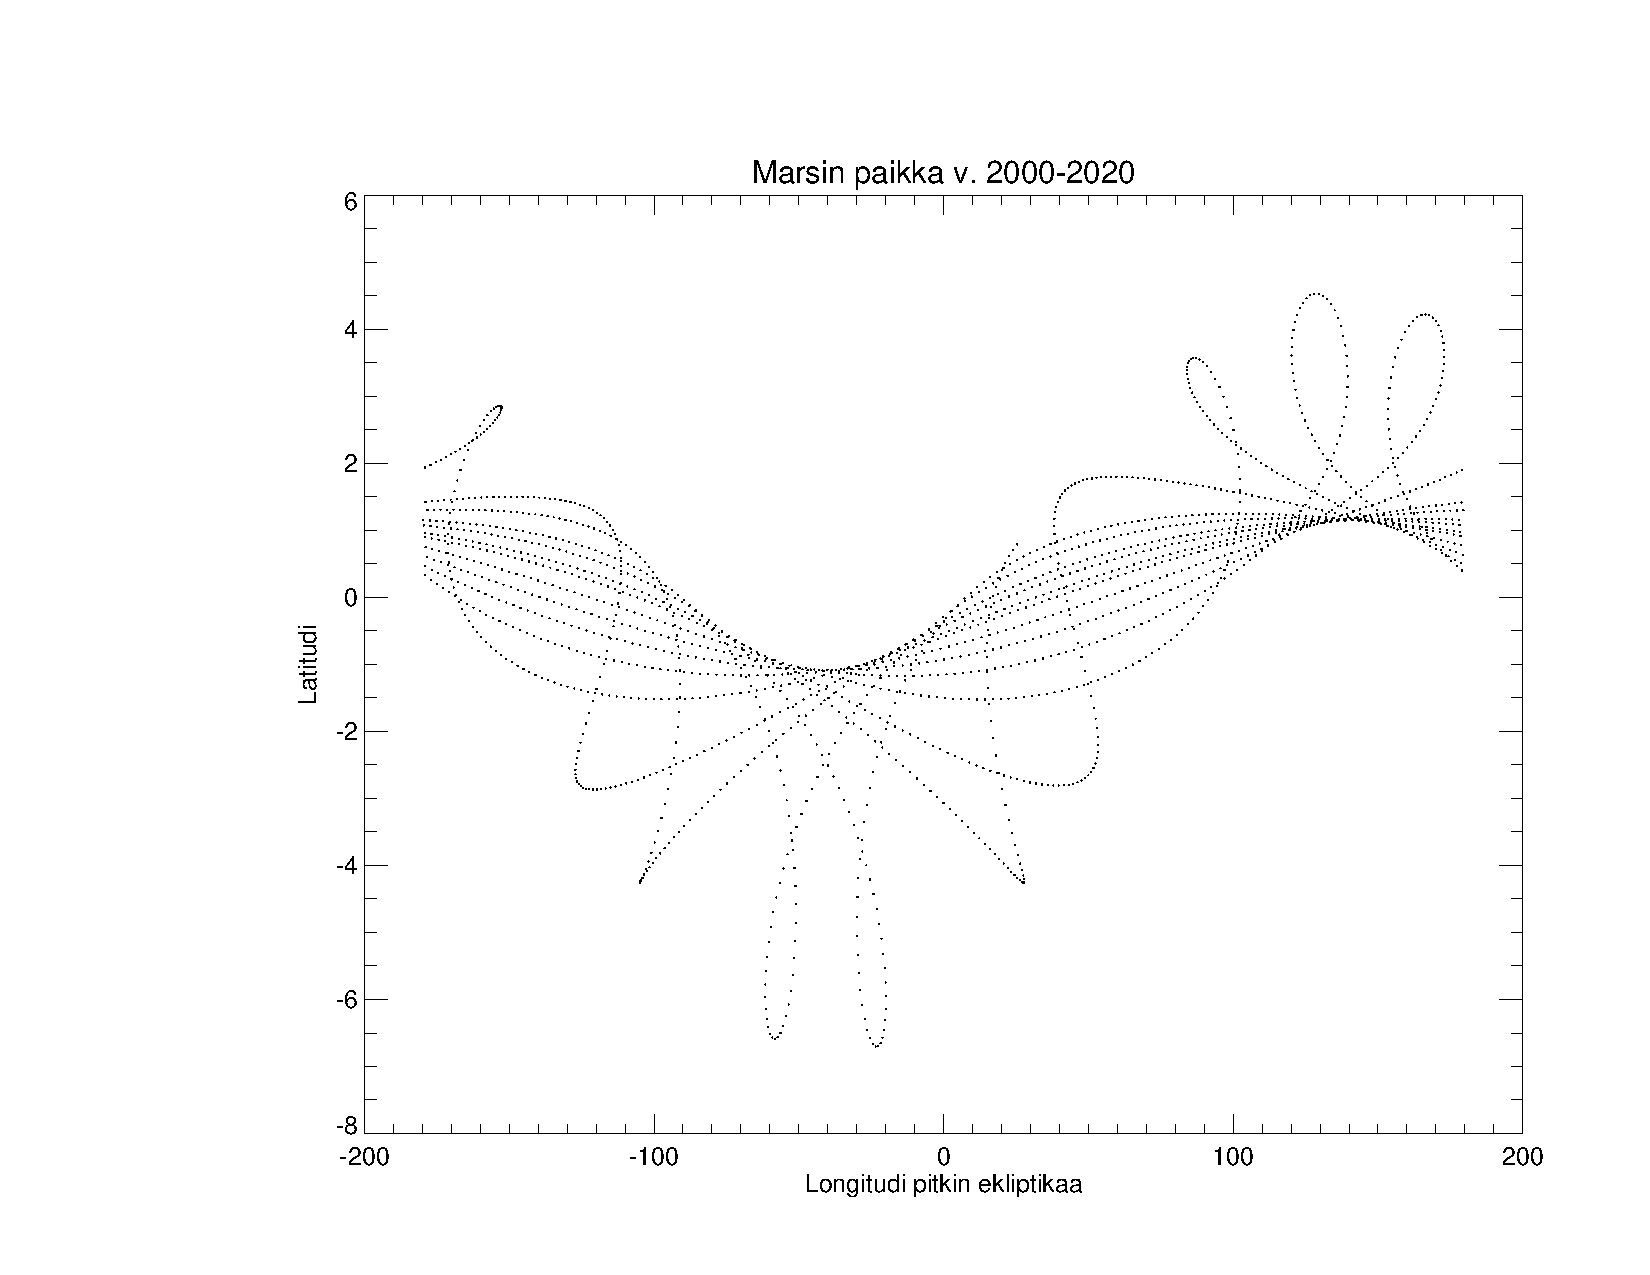
\includegraphics[angle=0,width=0.7\paperwidth]{ekliptikarata-1.pdf}
\caption{Marsin rata Maan ratatasokoordinaatistossa vuosina 2000-2020}
\label{Kuva1}
\end{figure}

\newpage
\subsection[Ekvaattorirata]{Marsin rata maan ekvaattoritasokoordinaatistossa}\label{Ekvaattori}

Maan päiväntasaajan suuntaisessa koordinaatistossa Marsin paikkaa ei voida yhtä yksikäsitteisen selkeästi esittää yhden kuvaajan avulla. Sen sijaan kuvassa \ref{Kuva2} on esitetty erikseen ohjelmassa mars\_oma.pro lasketut Marsin deklinaatio ja rektaskensio ajan funktiona.

Lisäksi saatuja laskennallisia arvoja verrattiin astro -kirjastosta saatuihin tarkkoihin arvoihin ja kuvassa \ref{Kuva2} esittettiin vastaavasti myös deklinaation ja rektaskension virheet ajan funktiona.

\begin{figure}[ht]
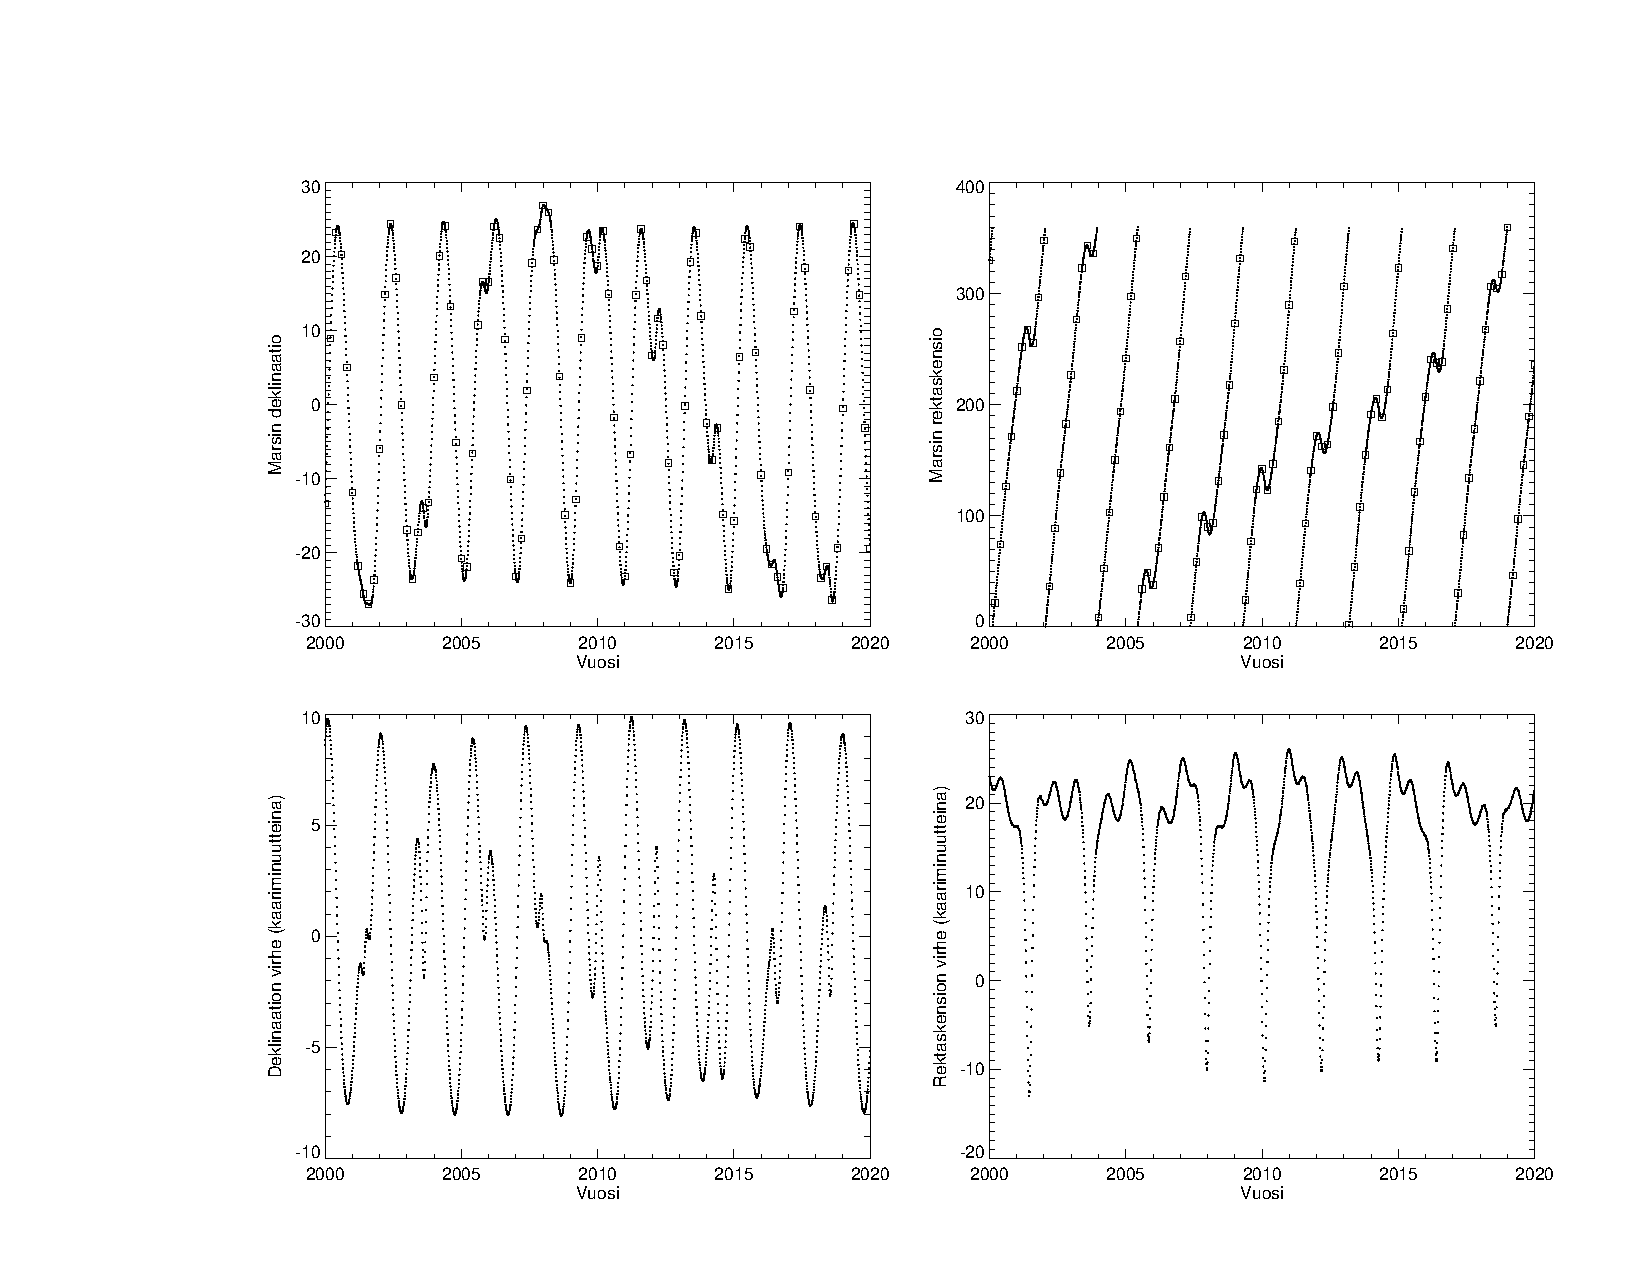
\includegraphics[angle=0,width=0.8\paperwidth]{deklinaatio-1.pdf}
\caption{Marsin deklinaatio ja rektaskensio sekä niiden virheet ajan funktiona.}
\label{Kuva2}
\end{figure}


\newpage
\subsection[Koodi1]{Ohjelman mars\_oma.pro sisältö}\label{Koodi1}
\begin{small}
\begin{verbatim}

program='mars_oma'

;----------------------------------------------------------------
;Taivaanmekaniikka 2012, kotitehtävä 1: Marsin sijainti taivaalla
;vuosina 2000-2020.
;----------------------------------------------------------------

;Tehdään taulukko 21 vuoden ajalle (ajanhetket 0.01 vuoden välein)

  timet=dindgen(2100)/100.      ;aika vuosina
  tday=timet*365.25d0           ;aika vuorokausina
  tcen=tday/36525.d0            ;aika vuosisatoina (juliaanista aikaa varten)

;Tehdään taulukot latitudia ja longitudia varten 
;(ekliptikasysteemi)

  lat_tab=timet
  lon_tab=timet

;Vastaavat taulukot deklinaatiota ja rektaskensiota varten
;(ekvaattorisysteemi)

  delta_tab=timet
  alpha_tab=timet

;Laitetaan juliaanisen kalenterin aika rullaamaan:

  for i=0l,n_elements(timet)-1 do begin

     T=tcen(i)

;----------------------------------------------------------------
;    MARSIN RATAELEMENTIT (aikakorjausten kanssa):
;----------------------------------------------------------------

     a=1.52366231-0.00007221*T        ;isoakselin puolikas
     ink=1.85061-25.47/3600.*T        ;inklinaatio
     wp=336.04084+1560.78/3600.*T     ;perihelin pituus (solmuviivasta)
     eks=0.09341233+0.00011902/3600*T ;eksentrisyys
     ome=49.57854-1020.19/3600*T      ;nousevan solmun pituus
     L=355.45332+0.52403304*tday(i)   ;keskipituus (solmuviivasta)


;Lasketaan näistä halutut suureet w ja M:

     w=wp-ome                   ;perisentrin argumentti
     M=L-wp                     ;keskianomalia

;Muutetaan keskianomalia vaihtelemaan välillä 0-2*Pi (rad)
;laskuvirheiden välttämiseksi

     M_mars=(M mod 360.d0)/360.d0*2.*!dpi

;-----------------------------------------------------------------
;Lasketaan rataelementeistä Marsin heliosentrinen radiusvektori
;rad_mars ohjelmalla elem_to_rv
;-----------------------------------------------------------------

;Määritetään aika tau nollaksi (käytetään keskianomaliaa M) 
;ja Marsin rataelementit vektoriksi elem_to_rv -ohjelmaa varten.

     tau=0.d0
     time=0.d0

     elem_mars=[a,eks,ink,ome,w,tau]

;Lasketaan Marsin heliosentrinen radiusvektori
     elem_to_rv,elem_mars,time,rad,vel,m0=M_mars
     rad_mars=rad

;-----------------------------------------------------------------
;    MAAN RATAELEMENTIT (aikakorjausten kanssa)
;-----------------------------------------------------------------

     a_maa=1.00000011-0.00000005*T      ;isoakselin puolikas
     ink_maa=0.00005-46.94/3600.*T      ;inklinaatio
     wp_maa=102.94719+1198.28/3600*T    ;perihelin pituus (solmuviivasta)
     eks_maa=0.01671022-0.00003804*T    ;eksentrisyys
     ome_maa=-11.26064-18228.25/3600.*T ;nousevan solmun pituus
     L_maa=100.46435+0.98560910*tday(i) ;keskipituus (solmuviivasta)

     w_maa=wp_maa-ome_maa       ;perisentrin argumentti
     M_m=L_maa-wp_maa           ;keskianomalia

;Muutetaan taas keskianomalia välille 0-2*Pi (rad)

     M_maa=(M_m mod 360.d0)/360.d0*2.*!dpi

;Maan heliosentrinen radiusvektori:

     elem_maa=[a_maa,eks_maa,ink_maa,ome_maa,w_maa,tau]

     elem_to_rv,elem_maa,time,rad,vel,M0=M_maa

     rad_maa=rad

;-----------------------------------------------------------------
;Maan ja Marsin radiusvektoreiden erotus 
;(siirretään origo Maahan; ekliptika-systeemi)
;-----------------------------------------------------------------

     x=rad_mars(0)-rad_maa(0)
     y=rad_mars(1)-rad_maa(1)
     z=rad_mars(2)-rad_maa(2)
     r=sqrt(x^2+y^2+z^2)

     lat_tab(i)=asin(z/r)*!radeg
     lon_tab(i)=atan(y,x)*!radeg

;------------------------------------------------------------------
;Siirrytään Maan ekvaattoritason suuntaiseen systeemiin:
;------------------------------------------------------------------

     ekli=23.4393           ;Maan akselin kallistuskulma
     sine=sin(ekli/!radeg)  ;Lasketaan valmiiksi kallistuskulman sini ja kosini
     cose=cos(ekli/!radeg)

;Marsin paikka ekvaattorisysteemissä
     xe=x
     ye=y*cose-z*sine
     ze=y*sine+z*cose

     re=sqrt(xe^2+ye^2+ze^2)    ;etäisyys
     delta=asin(ze/re)*!radeg   ;deklinaatio
     alpha=atan(ye,xe)*!radeg   ;rektaskensio

;Varmistetaan, että rektaskensio ei ole negatiivinen

     if(alpha le 0) then alpha=alpha+360

;Tallennetaan deklinaatio ja rektaskensio niille varattuihin
;taulukoihin ja suljetaan silmukka

     delta_tab(i)=delta
     alpha_tab(i)=alpha

  endfor

;---------------------------------------------------------------------
;Piirretään Marsin rata Maan ratatasokoordinaatistossa (v.2000-2020)
;---------------------------------------------------------------------

nwin
plot,lon_tab,lat_tab,xtitle='Longitudi pitkin ekliptikaa',$
title='Marsin paikka v. 2000-2020',ytitle='Latitudi',psym=3


;----------------------------------------------------------------------
;Plotataan samalle aikavälille deklinaatio ja inklinaatio ajan suhteen
;(Maan ekvaattoritason suuntainen koordinaatisto)
;----------------------------------------------------------------------

nwin
!p.multi=[0,2,2]
!p.charsize=0.7

;----------------------------------------------------------------------
;    DEKLINAATIO
;----------------------------------------------------------------------

;Ohjelmalla laskettu Marsin deklinaatio

plot,2000+timet,delta_tab,xr=[0,20]+2000,xtitle='Vuosi',$
ytitle='Marsin deklinaatio',psym=3


;Plotataan samaan kuvaan astro-kirjaston tarkkoja arvoja deklinaatiolle
;Käytetään tässä juliaanisen kalenterin aikoja, alkaen päivästä 1.1.2000
juldate,[2000.,1.,1],jd0
jd0=jd0+2400000.d0

jd=jd0+tday

planet_coords,jd,/jd,ra_astro,dec_astro,planet='mars'

;Plotataan vain joka 20. piste
index=lindgen(n_elements(timet)/20)*20
oplot,2000+timet(index),dec_astro(index),col=2,psym=6,syms=0.5


;----------------------------------------------------------------------
;      REKTASKENSIO
;----------------------------------------------------------------------

;Ohjelmalla laskettu Marsin rektaskensio

plot,2000+timet,alpha_tab,xr=[0,20]+2000,xtitle='Vuosi',$
ytitle='Marsin rektaskensio',psym=3

;Astro-kirjaston tarkkoja arvoja rektaskensiolle
oplot,2000+timet(index),ra_astro(index),col=2,psym=6,syms=0.5


;----------------------------------------------------------------------
;      VIRHEEN ARVIOINTI
;---------------------------------------------------------------------

;Määritetään deklinaation ja inklinaation virheet tarkkojen arvojen avulla.
;Käytetään nyt astron sijaan tarkkuudeltaan parempia JPL -ephemerideja.
planet_coords,jd,/jd,ra_jpl,dec_jpl,planet='mars',/jpl

;Deklinaation virhe
plot,2000+timet,(delta_tab-dec_jpl)*60.,xr=[0,20]+2000,$
xtitle='Vuosi',ytitle='Deklinaation virhe (kaariminuutteina)',psym=3


;Rektaskension virhe

;Varmistetaan ensin, että rektaskensiot alpha ja ra_jpl ovat samassa
;kierroksessa menossa (eivätkä poikkea toisistaan 2Pi verran)
d_alpha=atan(tan((alpha_tab-ra_jpl)/!radeg))*!radeg


plot,2000+timet,d_alpha*60,xr=[0,20]+2000,$
xtitle='Vuosi',ytitle='Rektaskension virhe (kaariminuutteina)',psym=3


  end


\end{verbatim}
\end{small}

\newpage

\section[Tehtävä 2]{Numeerinen integrointi}

\subsection[Tehtävä 2a]{Kahden kappaleen liike $1/r^2$ -voimakentässä}

\subsection[Tehtävä 2b]{Kahden kappaleen liike $1/r^3$ -voimakentässä}

\end{document}